\chapter{Results} \label{ch:results}
% \section{Metric Based Analysis}
% \section{Visual Based Analysis}
In line with the research questions, the evaluation section aims to quantify the performance gains obtained by using the Proxy Attention method. The section will compare the performance of networks that were trained with, and without Proxy Attention on the basis of classification metrics, and explainability improvements.

Note that complete performance logs can be found in the appendix.
\section{Accuracy}
This section explores the validation accuracy obtained by the models for different hyperparameters and datasets. Since the task at hand is a classification task, this measure is a direct comparison of the performance of the models.

\subsection{Results Per Dataset}
This subsection shows the accuracies per model for each dataset. Tabulated results can be found in the appendix in Table ~\ref{tab:summary_ds}.

\subsubsection{Dogs Results}
This section shows the accuracies per model for the Dogs dataset. The results are shown in Figure \ref{fig:dogs_results}. 
\begin{figure}[H]
    \centering
    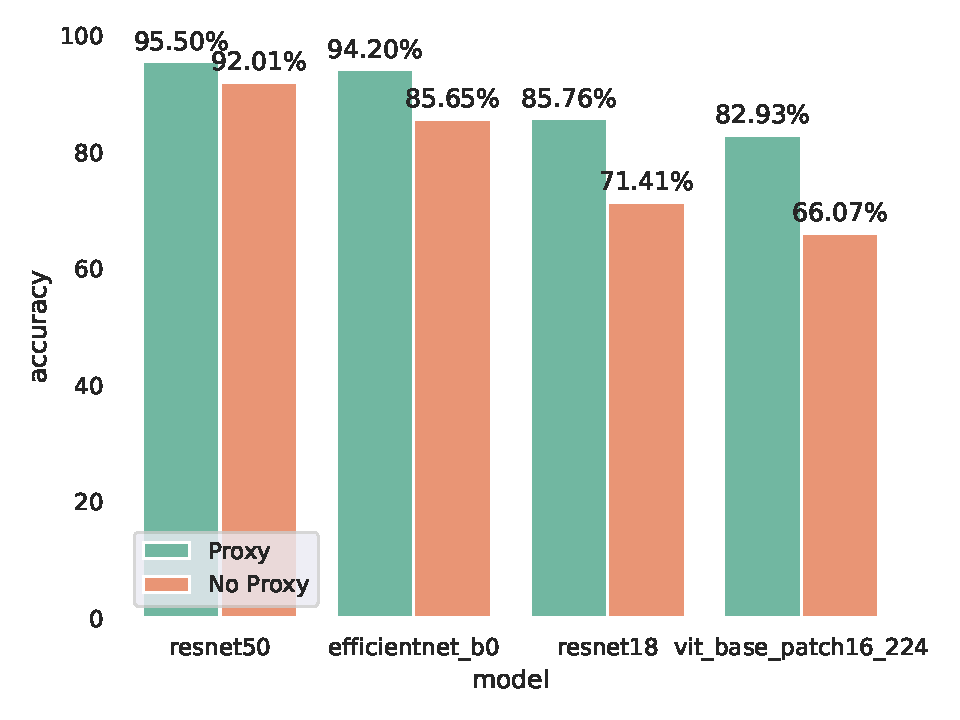
\includegraphics[width=1\textwidth]{results/dogs_results.pdf}
    \caption{Comparing Accuracies of models trained with and without Proxy Attention on the Dogs dataset}
    \label{fig:dogs_results}
\end{figure}

\subsection{Cifar100 Results}
This section shows the accuracies per model for the Cifar100 dataset. The results are shown in Figure \ref{fig:cifar100_results}. 
\begin{figure}[H]
    \centering
    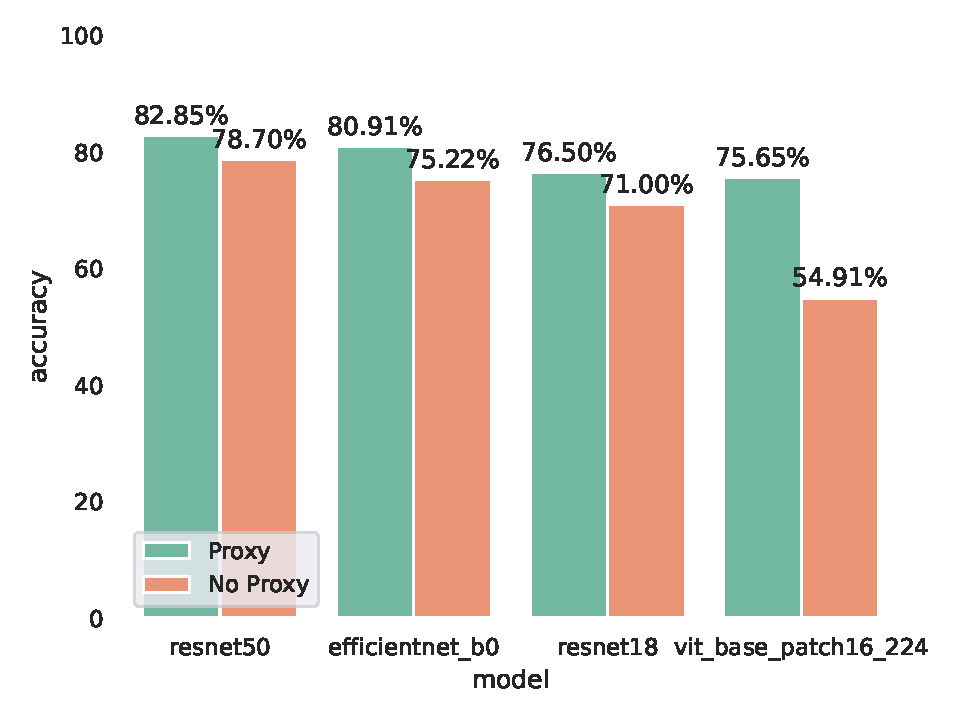
\includegraphics[width=1\textwidth]{results/cifar100_results.pdf}
    \caption{Comparing Accuracies of models trained with and without Proxy Attention on the Cifar100 dataset}
    \label{fig:cifar100_results}
\end{figure}

\subsection{Caltech101 Results}
This section shows the accuracies per model for the Caltech101 dataset. The results are shown in Figure \ref{fig:caltech101_results}. 
\begin{figure}[H]
    \centering
    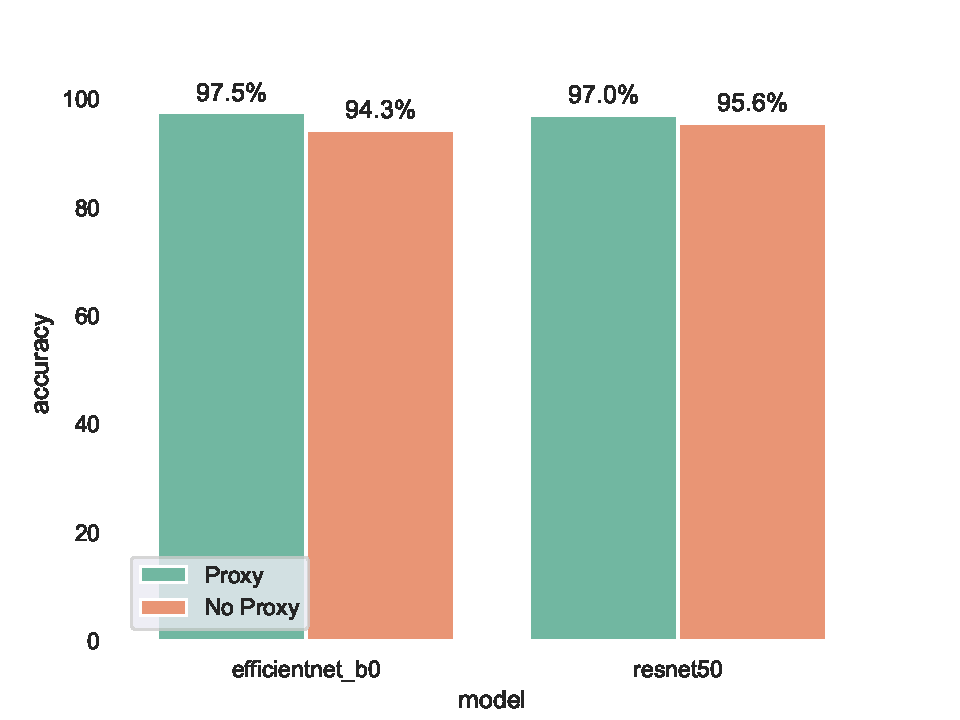
\includegraphics[width=1\textwidth]{results/caltech101_results.pdf}
    \caption{Comparing Accuracies of models trained with and without Proxy Attention on the Caltech101 dataset}
    \label{fig:caltech101_results}
\end{figure}

\subsection{Asl Results}
This section shows the accuracies per model for the Asl dataset. The results are shown in Figure \ref{fig:asl_results}. 
\begin{figure}[H]
    \centering
    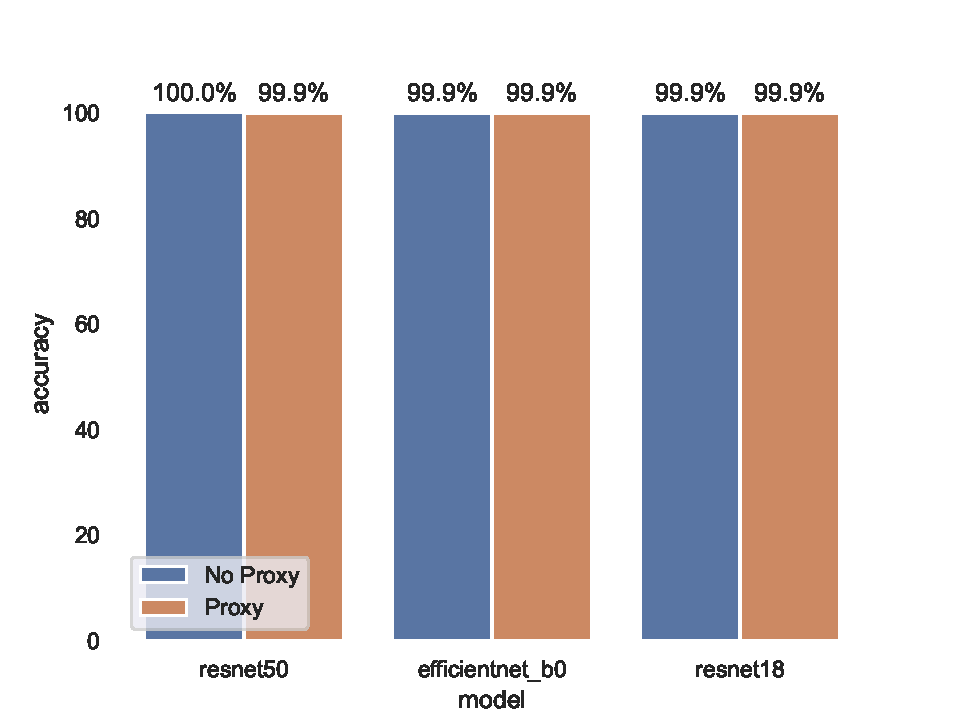
\includegraphics[width=1\textwidth]{results/asl_results.pdf}
    \caption{Comparing Accuracies of models trained with and without Proxy Attention on the Asl dataset}
    \label{fig:asl_results}
\end{figure}

\subsection{Plantdisease Results}
This section shows the accuracies per model for the Plantdisease dataset. The results are shown in Figure \ref{fig:plantdisease_results}. 
\begin{figure}[H]
    \centering
    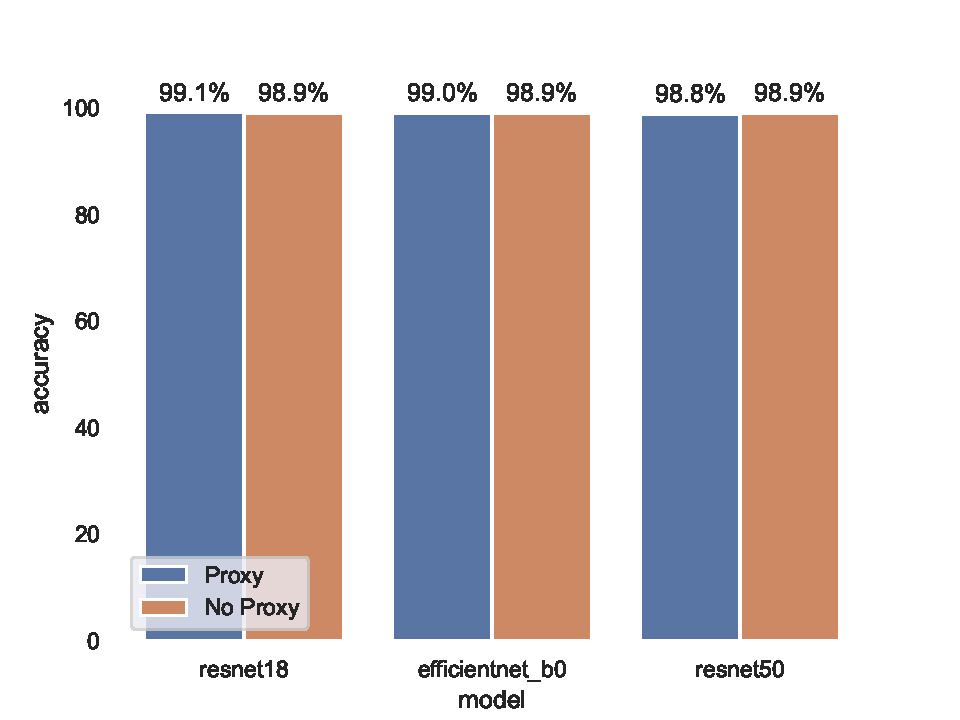
\includegraphics[width=1\textwidth]{results/plantdisease_results.pdf}
    \caption{Comparing Accuracies of models trained with and without Proxy Attention on the Plantdisease dataset}
    \label{fig:plantdisease_results}
\end{figure}

\subsection{Results Grouped By Schedule}
This section explores the validation accuracy obtained for different step schedules. The results are shown in Figure \ref{fig:schedresnet50_results}. 
\begin{figure}[H]
    \centering
    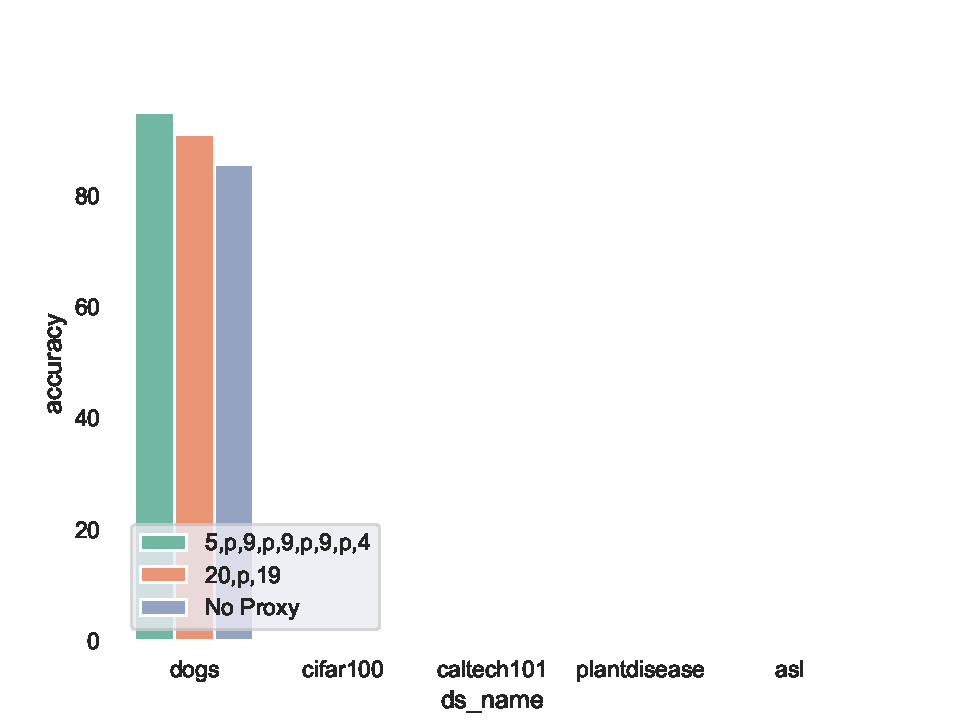
\includegraphics[width=1\textwidth]{results/schedule_resnet50.pdf}
    \caption{Comparing Accuracies of models trained with and without Proxy Attention on the ResNet50 \cite{heDeepResidualLearning2016} architecture for different step schedules}.
    \label{fig:schedresnet50_results}
\end{figure}

\subsection{Results Grouped By Proxy Threshold}
This section explores the validation accuracy obtained for different Proxy thresholds. The results are shown in Figure \ref{fig:proxy_threshold}. 
\begin{figure}[H]
    \centering
    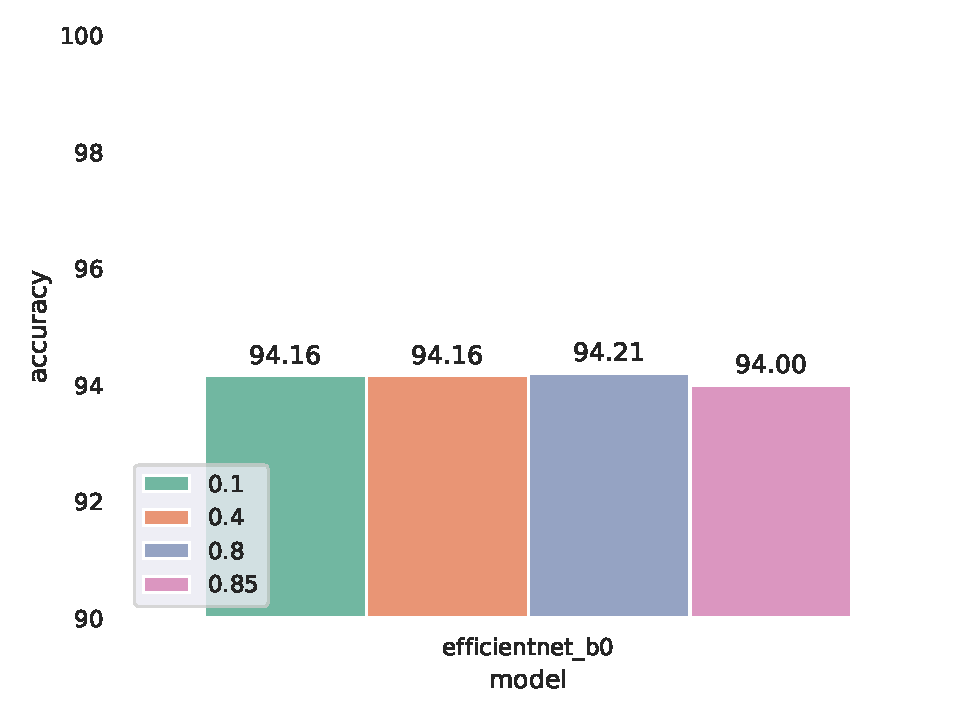
\includegraphics[width=1\textwidth]{results/proxy_threshold_results.pdf}
    \caption{Comparing Accuracies of models trained with and without Proxy Attention on the EfficientNetB0 \cite{tanEfficientnetRethinkingModel2019} architectures for different Proxy Thresholds}
    \label{fig:proxy_threshold}
\end{figure}

\subsection{Results Grouped By Proxy Image Weight}
This section explores the validation accuracy obtained for different Proxy image weights. The results are shown in Figure \ref{fig:proxy_weight}. 
\begin{figure}[H]
    \centering
    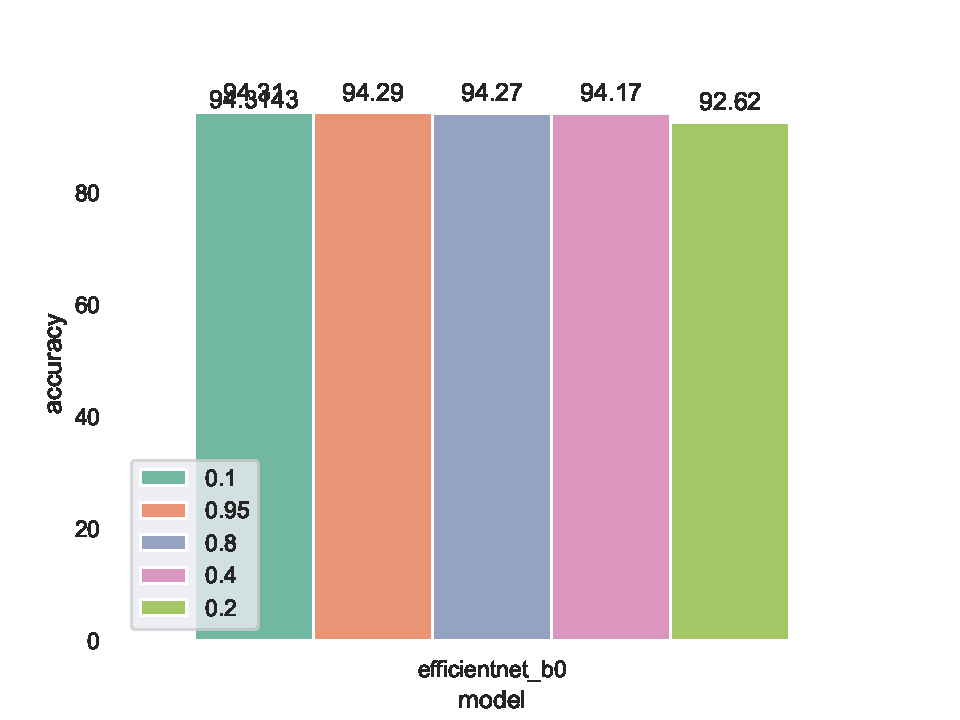
\includegraphics[width=1\textwidth]{results/proxy_weight_results.pdf}
    \caption{Comparing Accuracies of models trained with and without Proxy Attention on the EfficientNetB0 \cite{tanEfficientnetRethinkingModel2019} architectures for different Proxy Image Weights}
    \label{fig:proxy_weight}
\end{figure}



\section{Explanability}
This section explores the explainability of the models for different hyperparameters and datasets by using a trained model to generate attention maps for a given input image. The attention maps are compared between the same network (with the same hyperparameters) trained with and without Proxy Attention.

\subsection{CIFAR 100, ResNet18}

    \begin{figure}[H]
        \centering
        \begin{subfigure}[b]{1\textwidth}
            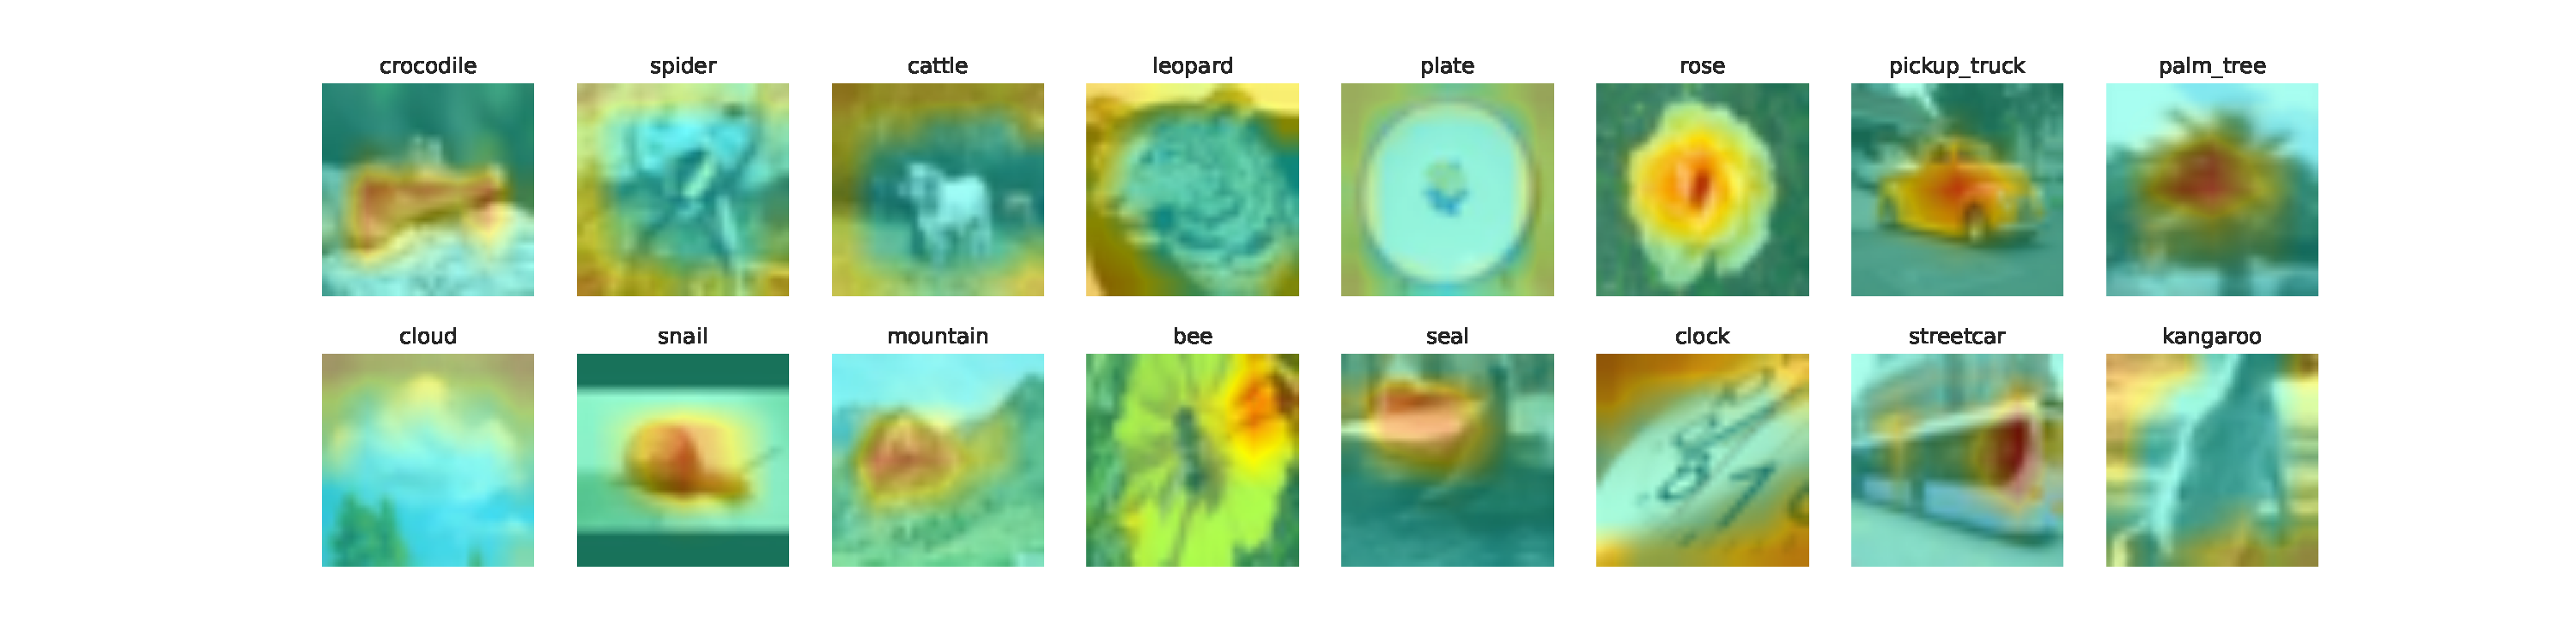
\includegraphics[width=\textwidth]{images/cifar100_resnet18_noproxy_0.pdf}
            \caption{Without Proxy Attention}
        \end{subfigure}
        \hfill
        \begin{subfigure}[b]{1\textwidth}
            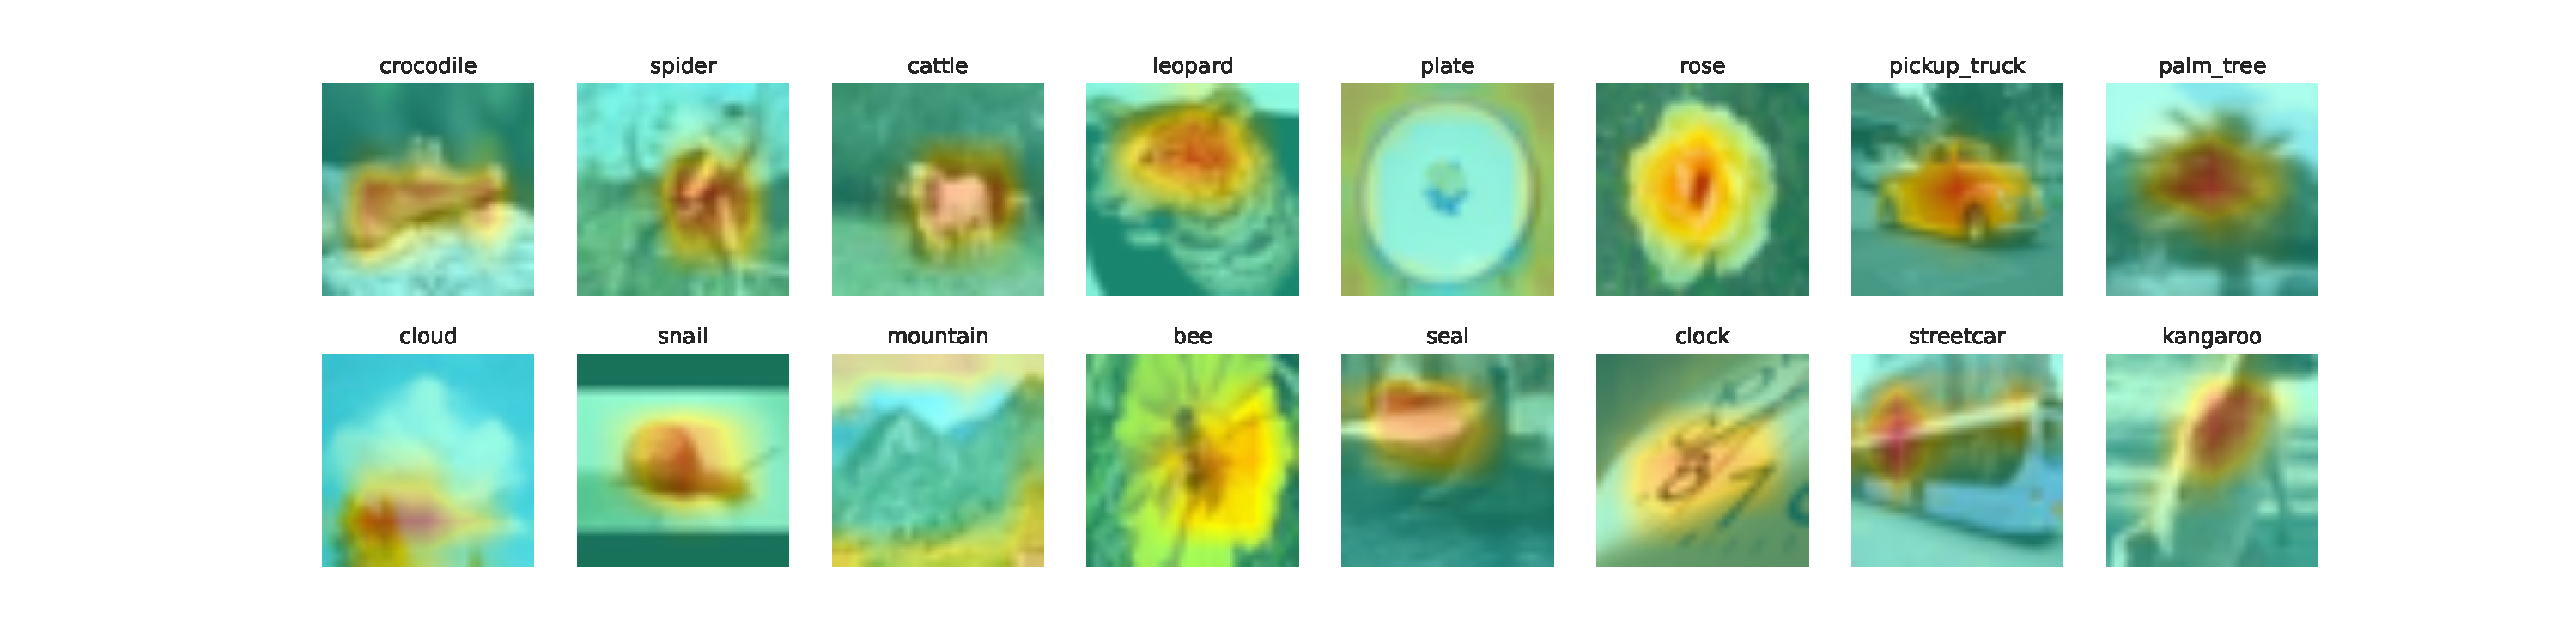
\includegraphics[width=\textwidth]{images/cifar100_resnet18_proxy_0.pdf}
            \caption{With Proxy Attention}
        \end{subfigure}
        \caption{Comparison of attention maps generated by resnet18 trained with and without Proxy Attention on the cifar100 dataset}
    \end{figure}
    

    \begin{figure}[H]
        \centering
        \begin{subfigure}[b]{1\textwidth}
            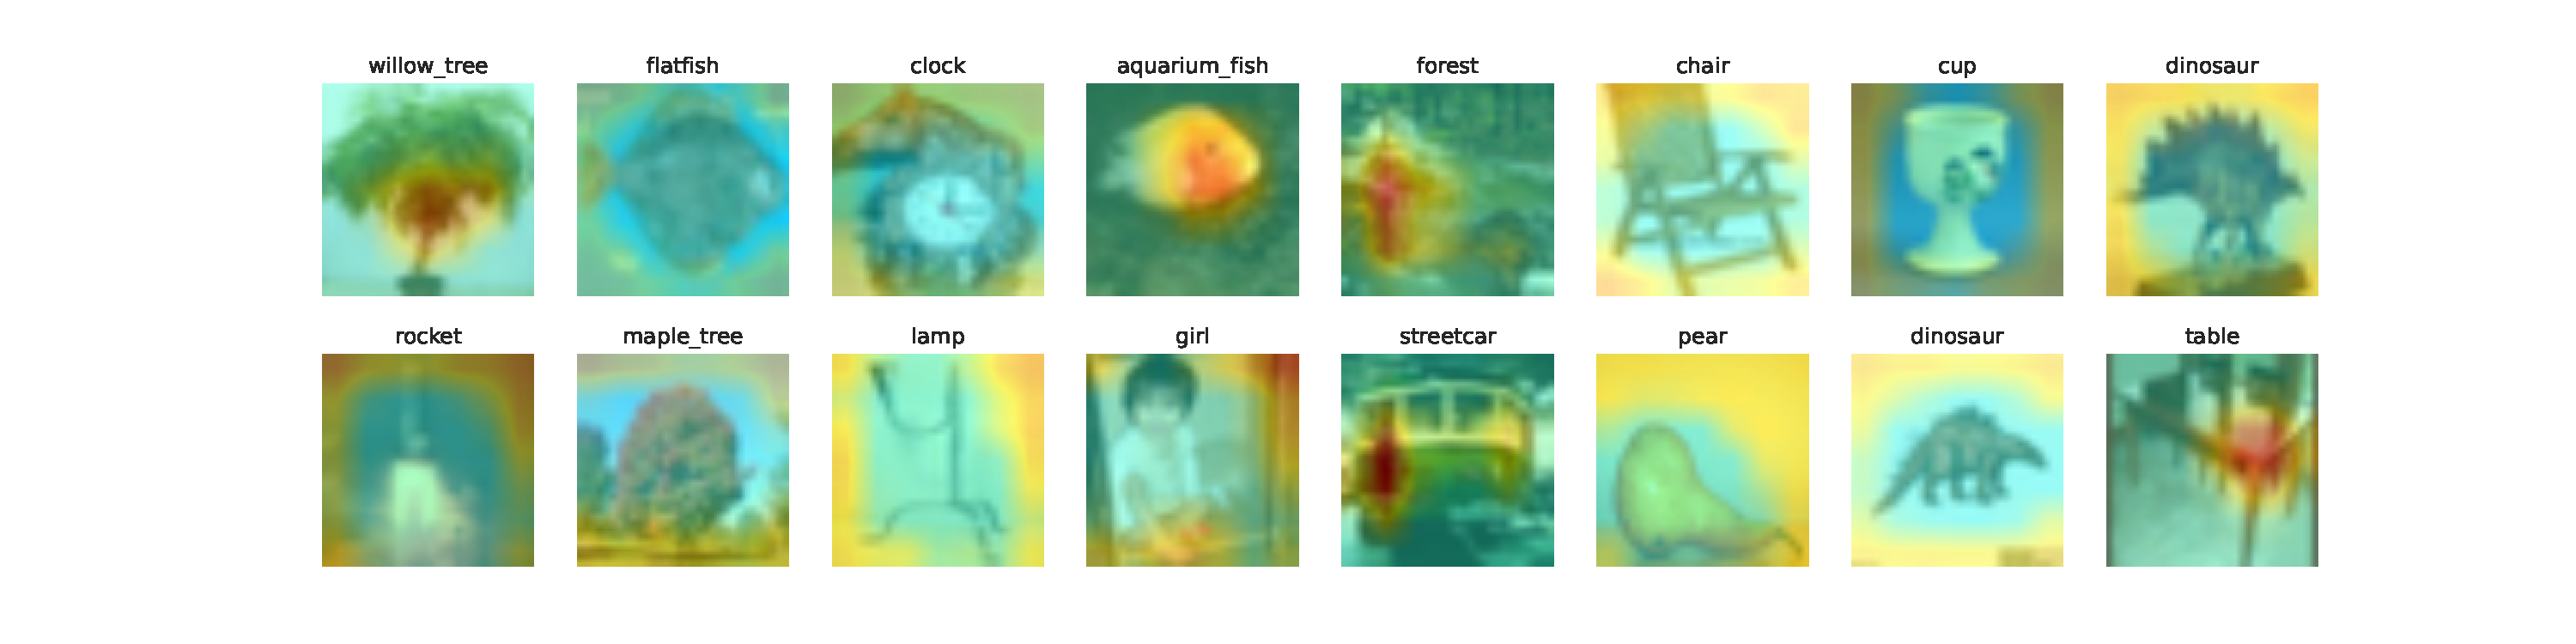
\includegraphics[width=\textwidth]{images/cifar100_resnet18_noproxy_1.pdf}
            \caption{Without Proxy Attention}
        \end{subfigure}
        \hfill
        \begin{subfigure}[b]{1\textwidth}
            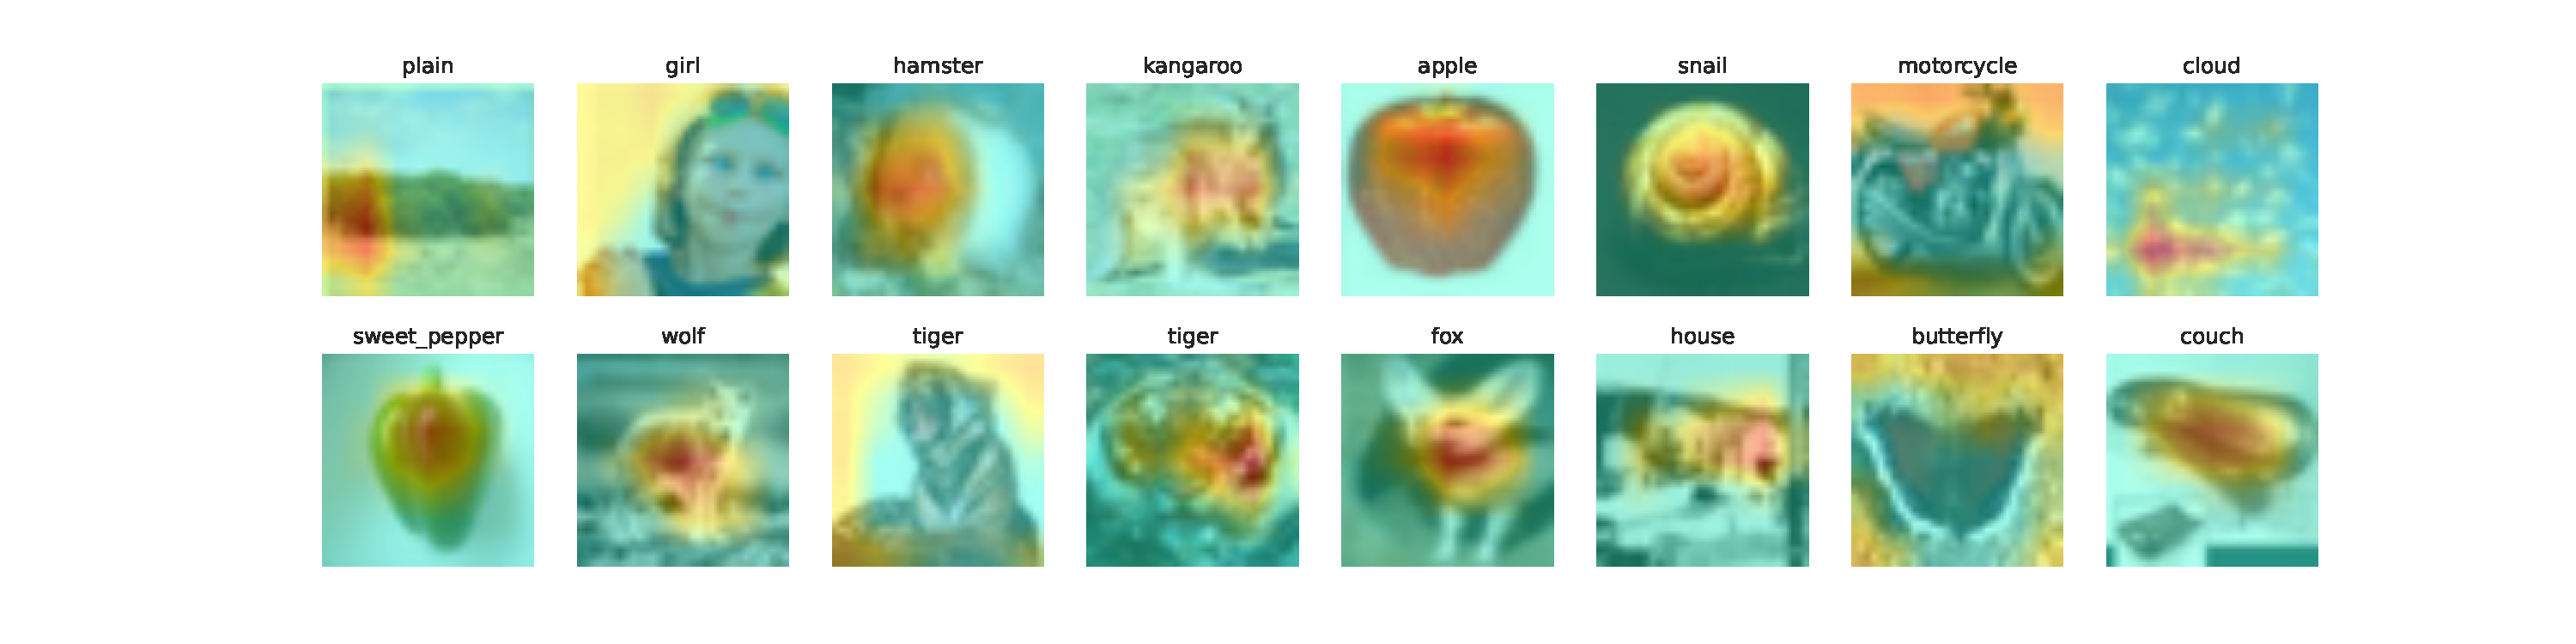
\includegraphics[width=\textwidth]{images/cifar100_resnet18_proxy_1.pdf}
            \caption{With Proxy Attention}
        \end{subfigure}
        \caption{Comparison of attention maps generated by resnet18 trained with and without Proxy Attention on the cifar100 dataset}
    \end{figure}
    

    \begin{figure}[H]
        \centering
        \begin{subfigure}[b]{1\textwidth}
            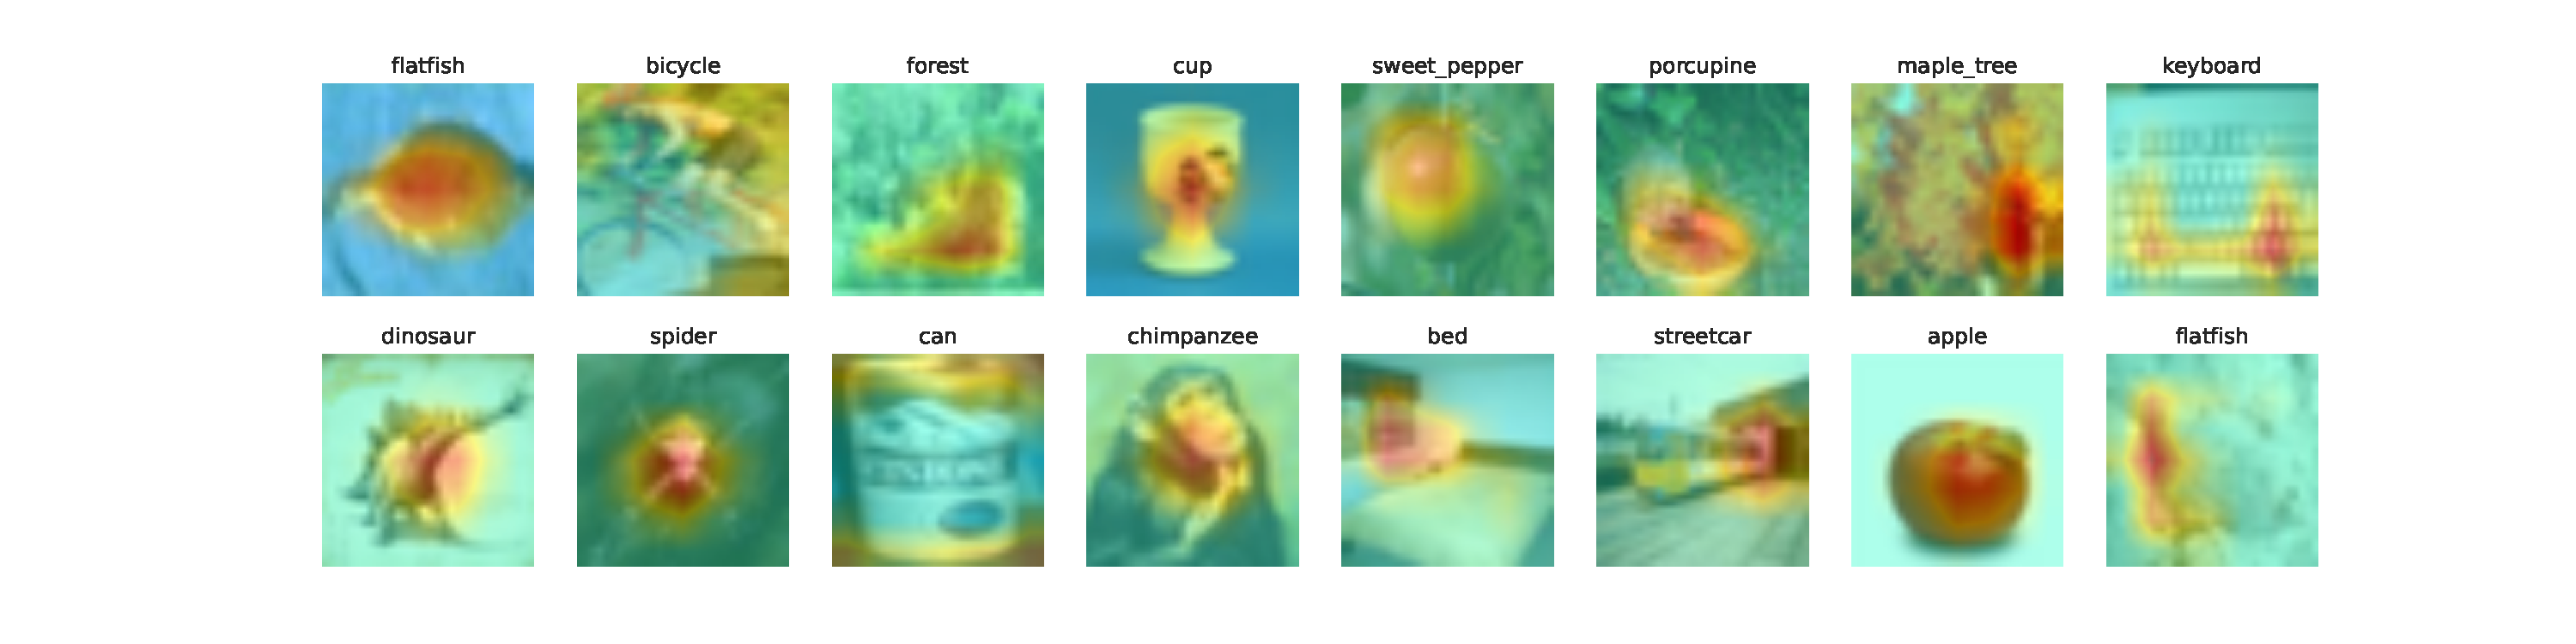
\includegraphics[width=\textwidth]{images/cifar100_resnet18_noproxy_2.pdf}
            \caption{Without Proxy Attention}
        \end{subfigure}
        \hfill
        \begin{subfigure}[b]{1\textwidth}
            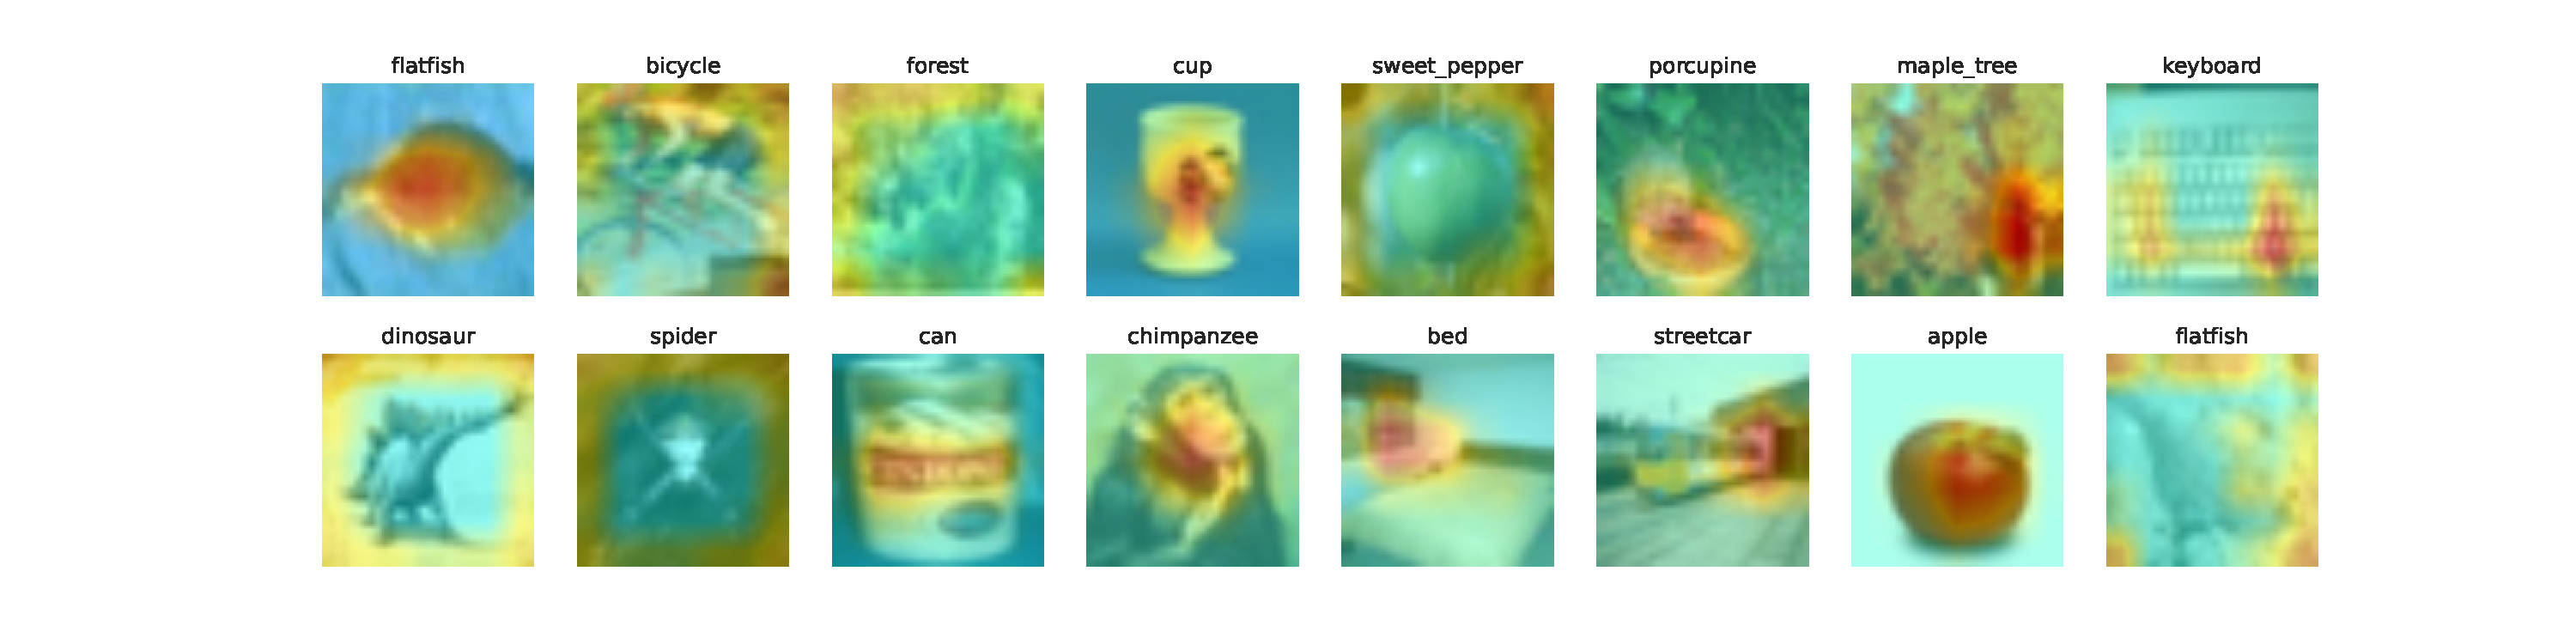
\includegraphics[width=\textwidth]{images/cifar100_resnet18_proxy_2.pdf}
            \caption{With Proxy Attention}
        \end{subfigure}
        \caption{Comparison of attention maps generated by resnet18 trained with and without Proxy Attention on the cifar100 dataset}
    \end{figure}
    

    \begin{figure}[H]
        \centering
        \begin{subfigure}[b]{1\textwidth}
            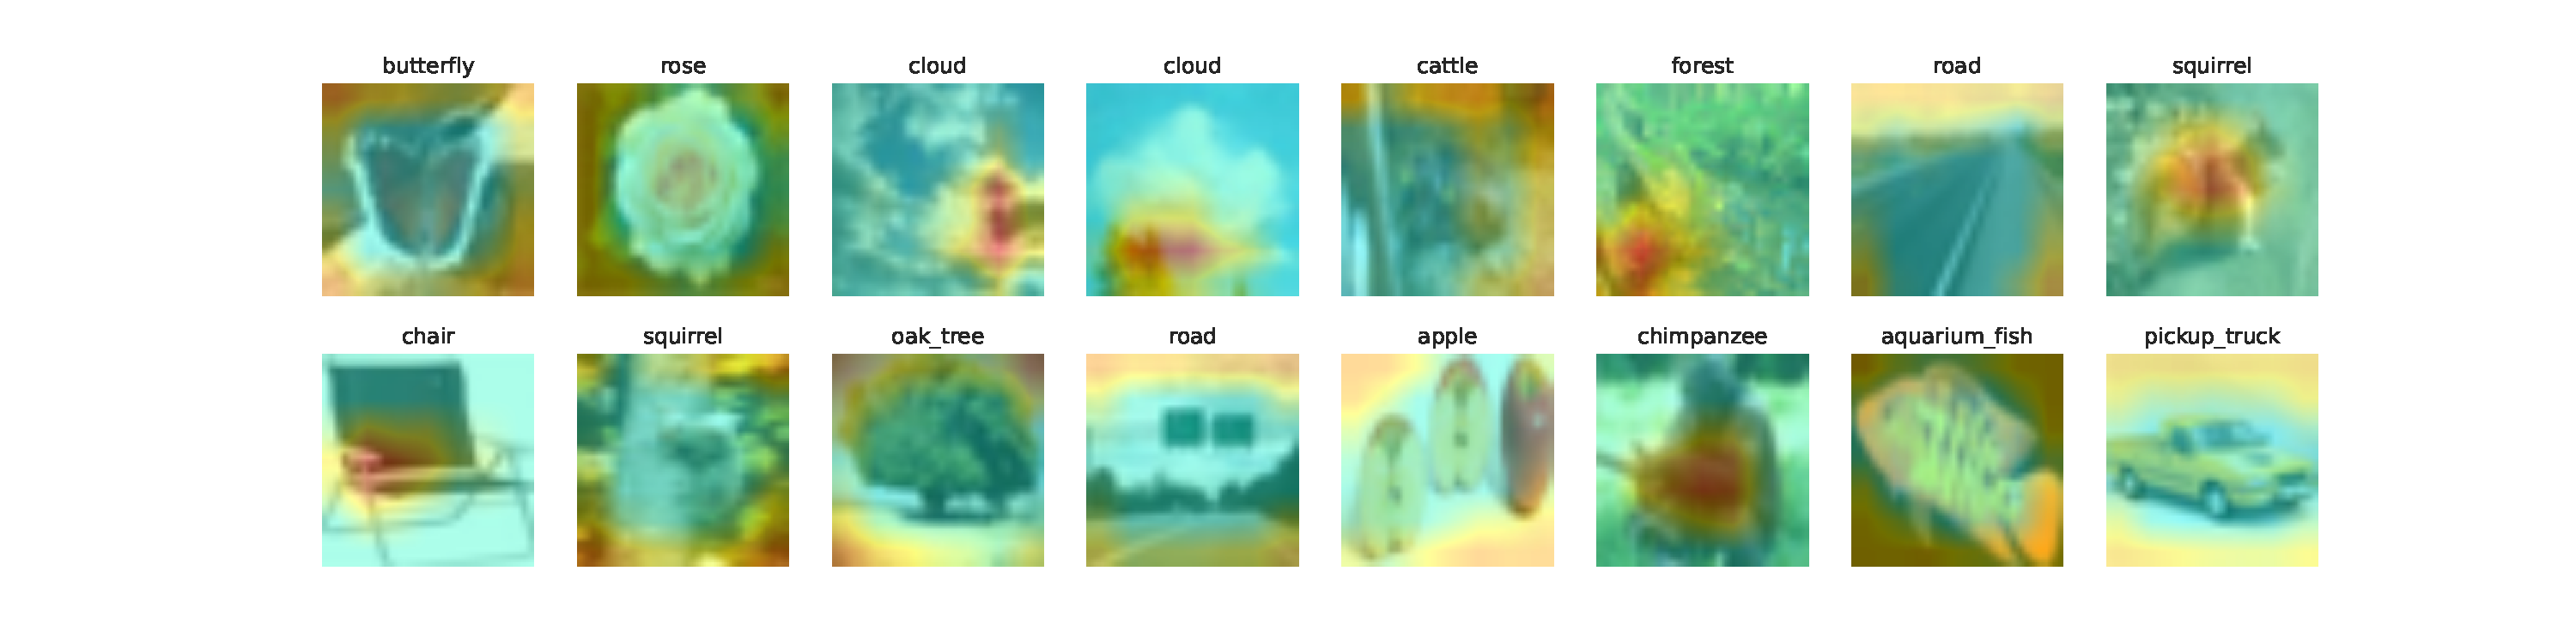
\includegraphics[width=\textwidth]{images/cifar100_resnet18_noproxy_3.pdf}
            \caption{Without Proxy Attention}
        \end{subfigure}
        \hfill
        \begin{subfigure}[b]{1\textwidth}
            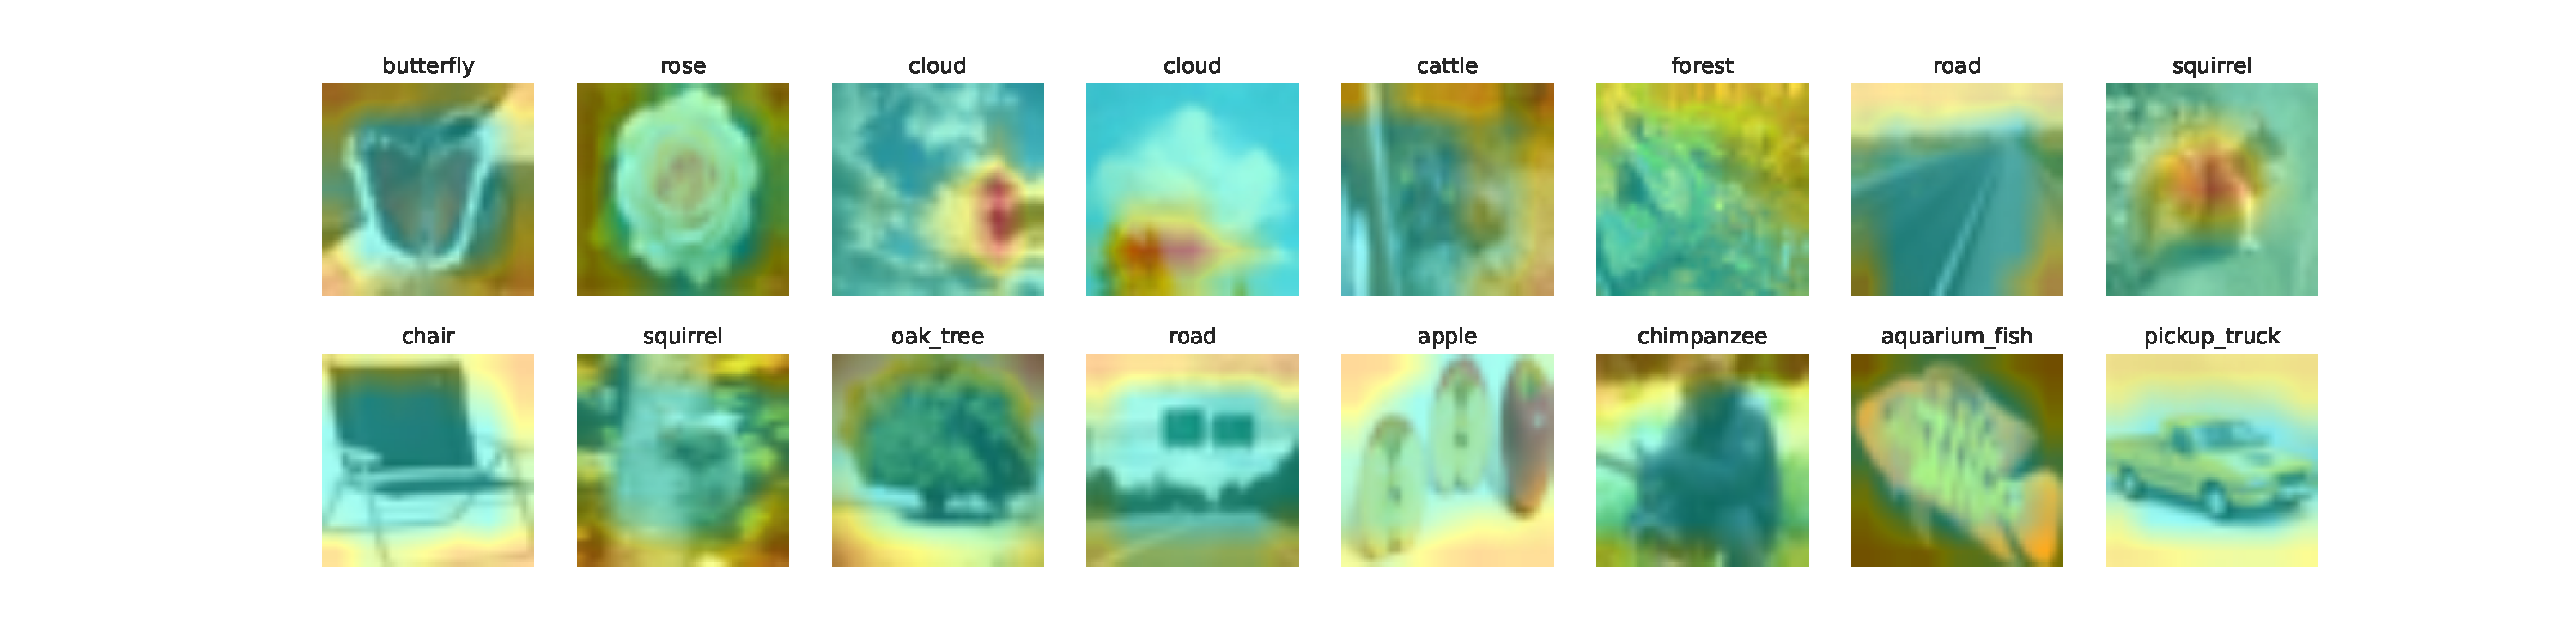
\includegraphics[width=\textwidth]{images/cifar100_resnet18_proxy_3.pdf}
            \caption{With Proxy Attention}
        \end{subfigure}
        \caption{Comparison of attention maps generated by resnet18 trained with and without Proxy Attention on the cifar100 dataset}
    \end{figure}
    


\subsection{CIFAR 100, EfficientNetB0}

    \begin{figure}[H]
        \centering
        \begin{subfigure}[b]{1\textwidth}
            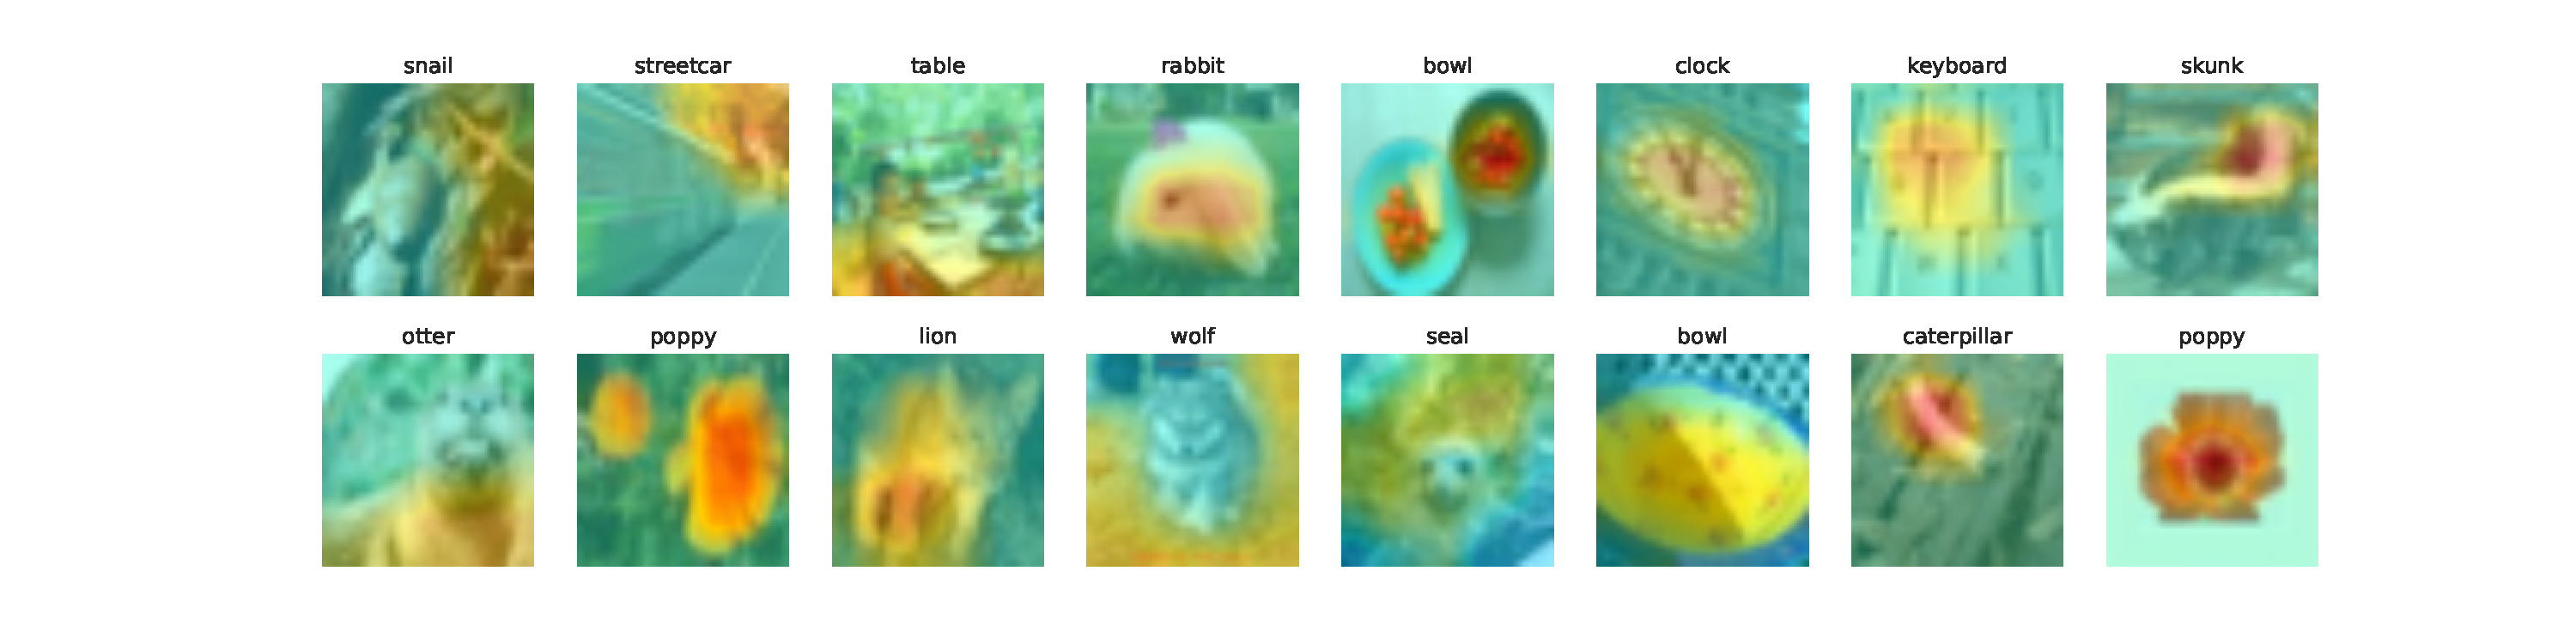
\includegraphics[width=\textwidth]{images/cifar100_efficientnet_b0_noproxy_0.pdf}
            \caption{Without Proxy Attention}
        \end{subfigure}
        \hfill
        \begin{subfigure}[b]{1\textwidth}
            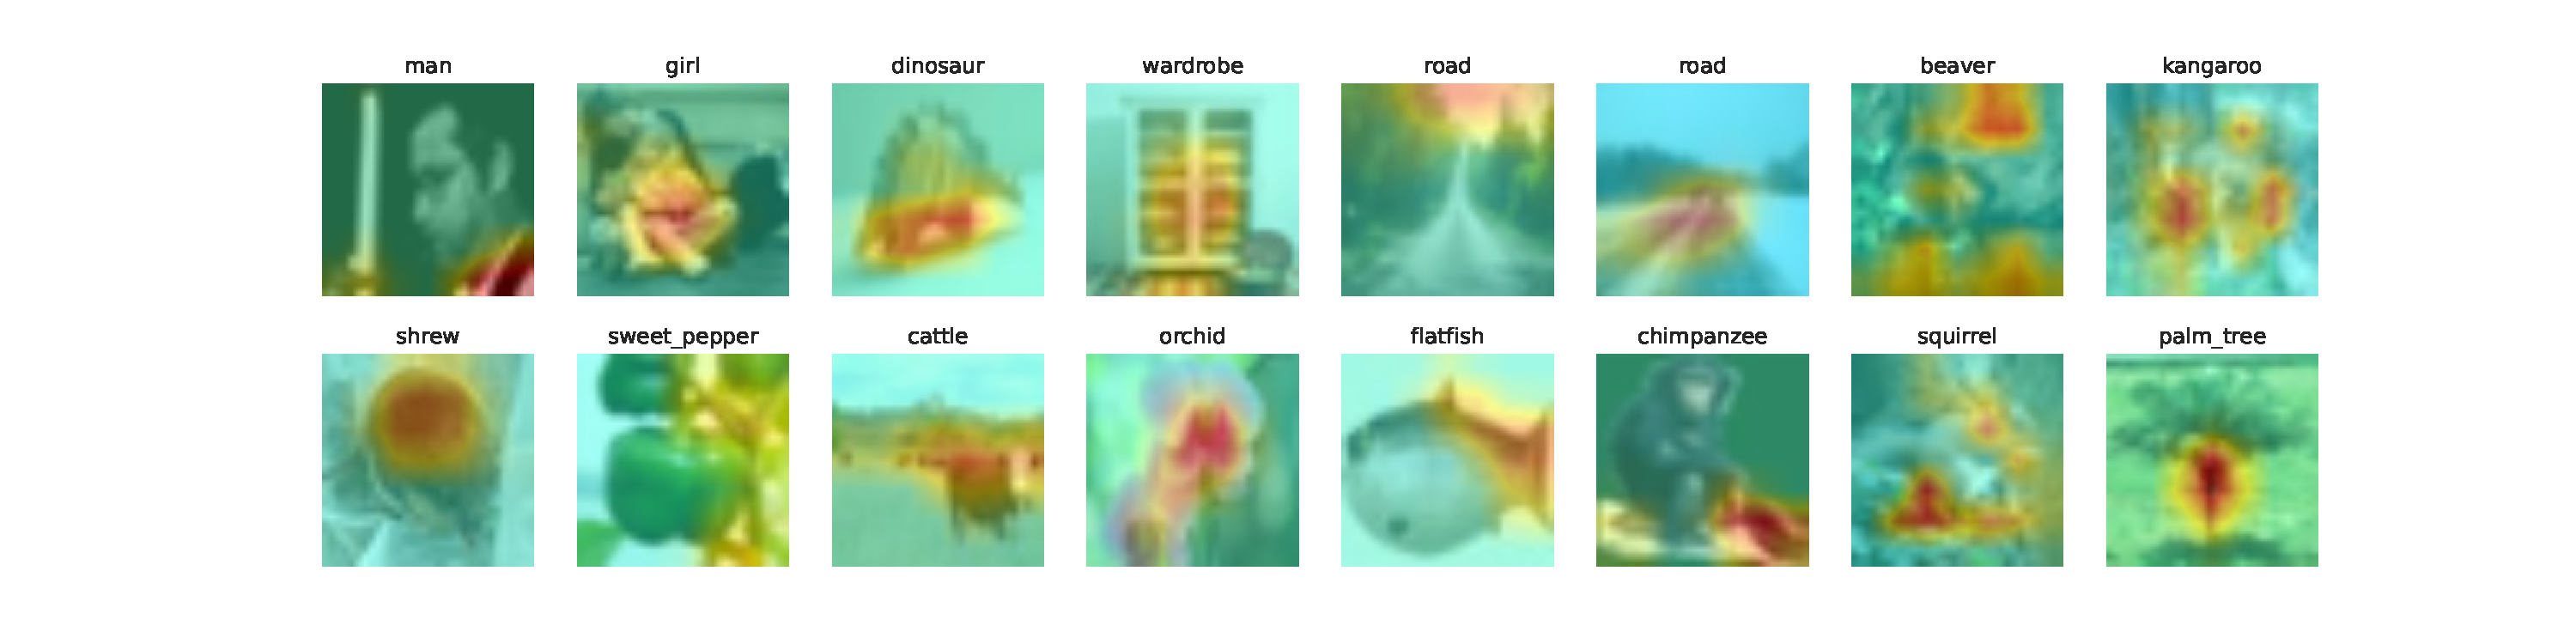
\includegraphics[width=\textwidth]{images/cifar100_efficientnet_b0_proxy_0.pdf}
            \caption{With Proxy Attention}
        \end{subfigure}
        \caption{Comparison of attention maps generated by efficientnet\_b0 trained with and without Proxy Attention on the cifar100 dataset}
    \end{figure}
    

    \begin{figure}[H]
        \centering
        \begin{subfigure}[b]{1\textwidth}
            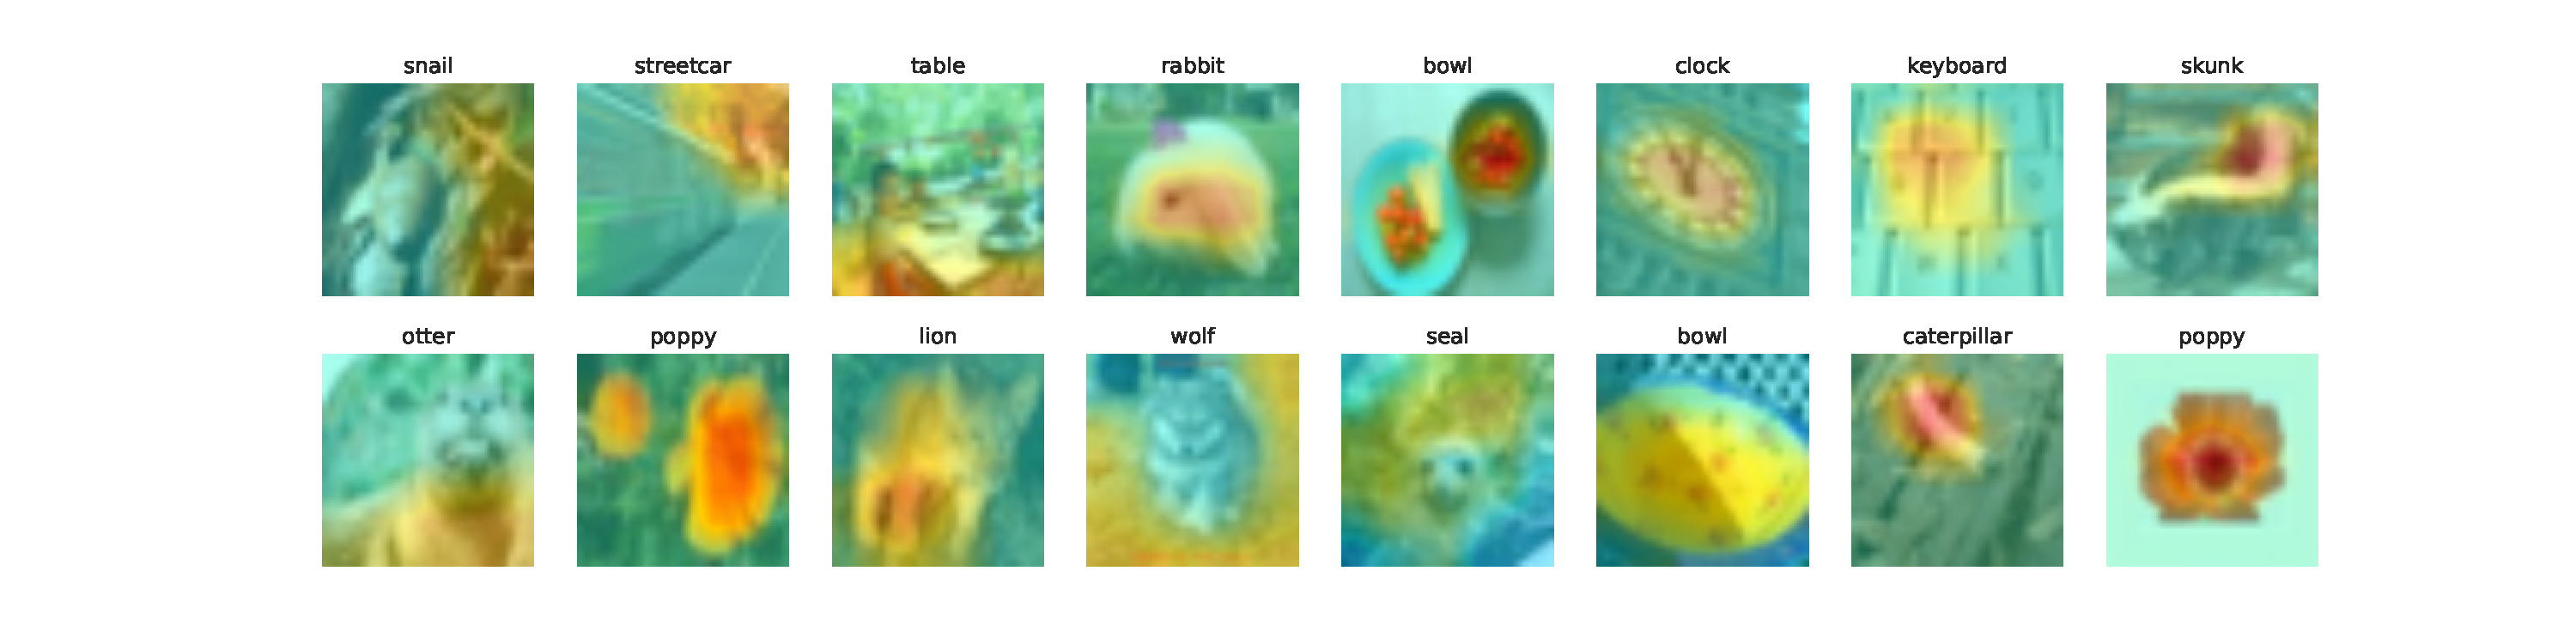
\includegraphics[width=\textwidth]{images/cifar100_efficientnet_b0_noproxy_0.pdf}
            \caption{Without Proxy Attention}
        \end{subfigure}
        \hfill
        \begin{subfigure}[b]{1\textwidth}
            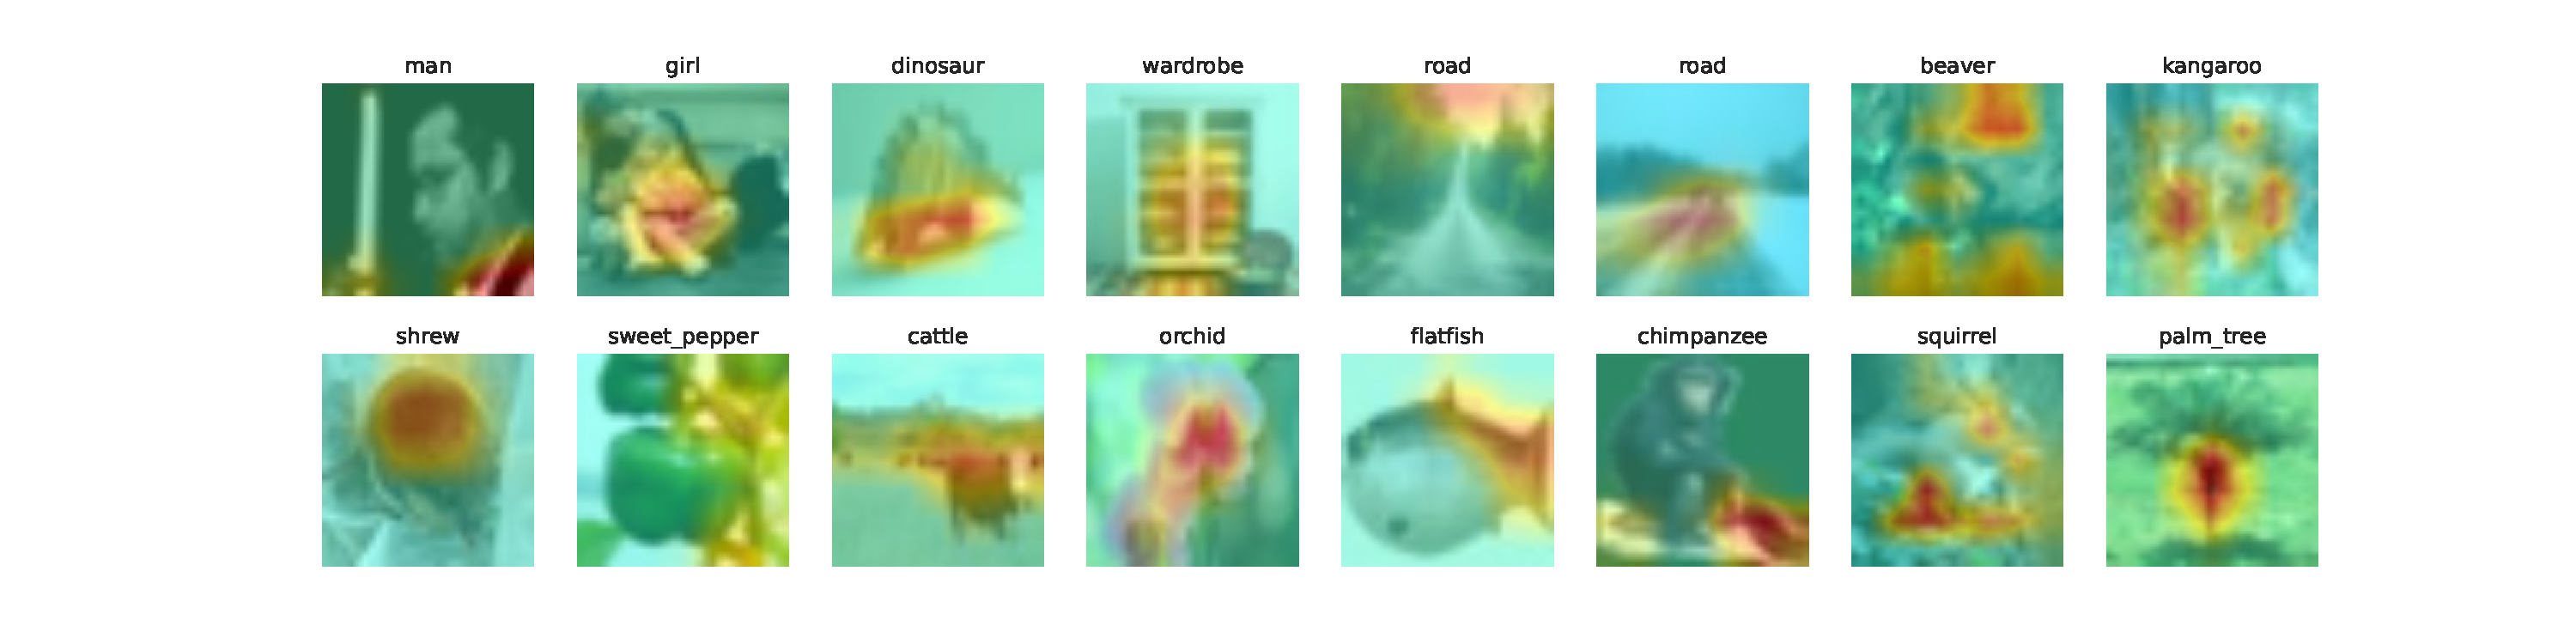
\includegraphics[width=\textwidth]{images/cifar100_efficientnet_b0_proxy_0.pdf}
            \caption{With Proxy Attention}
        \end{subfigure}
        \caption{Comparison of attention maps generated by efficientnet\_b0 trained with and without Proxy Attention on the cifar100 dataset}
    \end{figure}
    

    \begin{figure}[H]
        \centering
        \begin{subfigure}[b]{1\textwidth}
            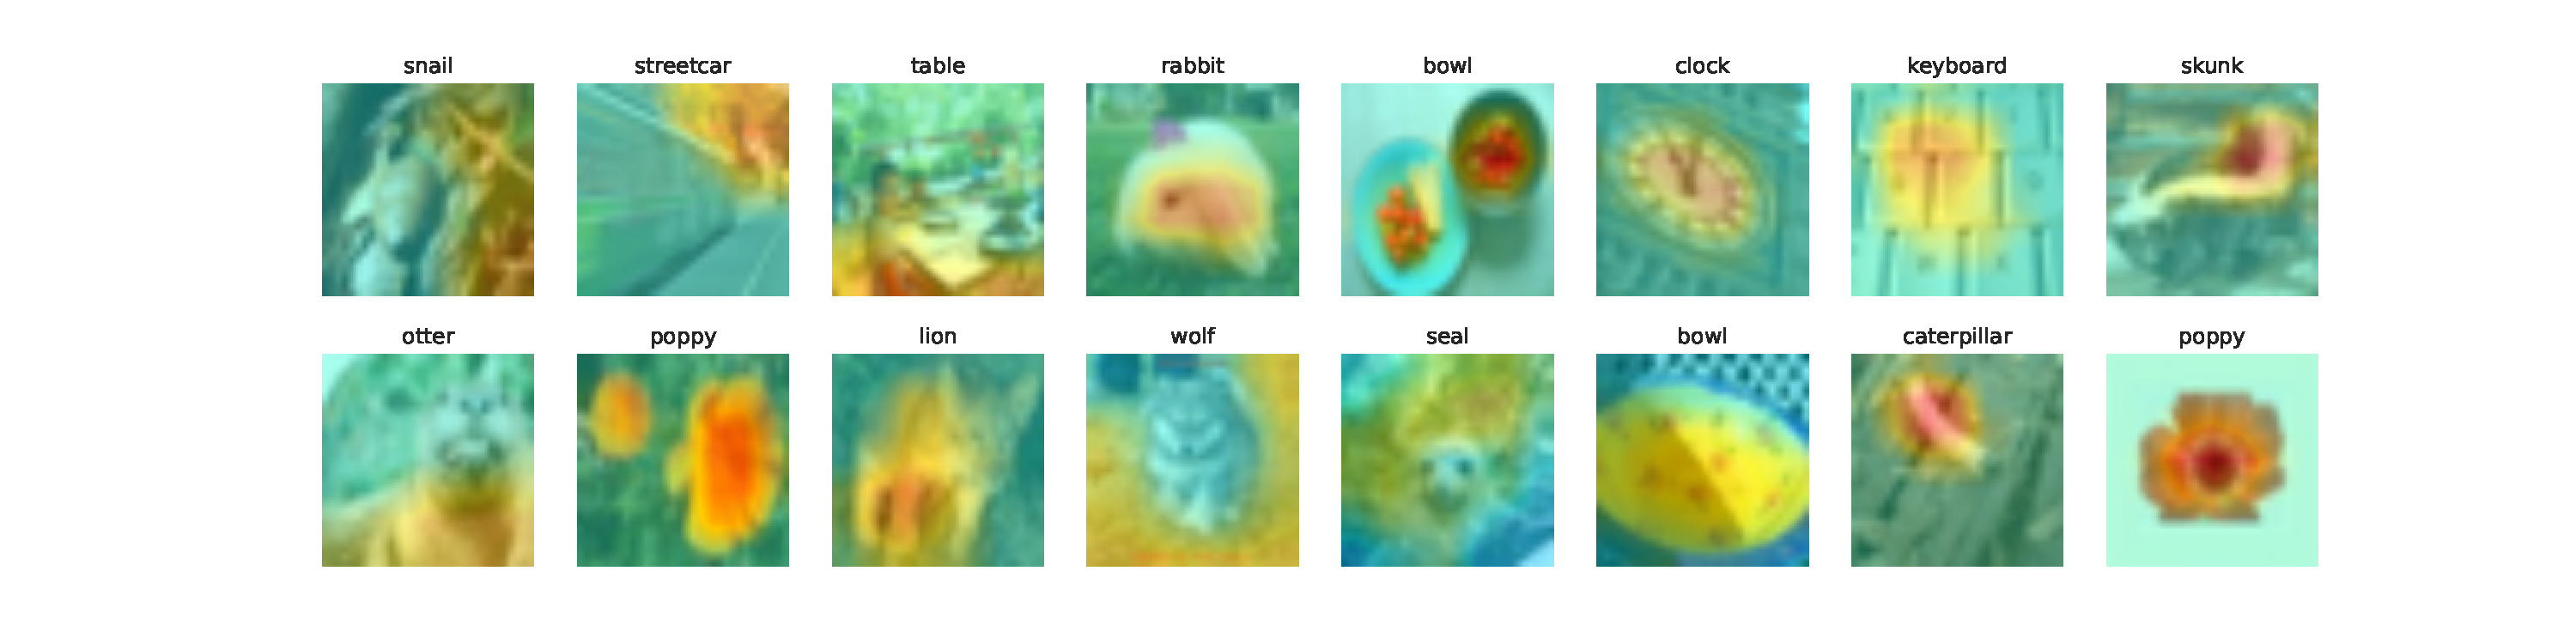
\includegraphics[width=\textwidth]{images/cifar100_efficientnet_b0_noproxy_0.pdf}
            \caption{Without Proxy Attention}
        \end{subfigure}
        \hfill
        \begin{subfigure}[b]{1\textwidth}
            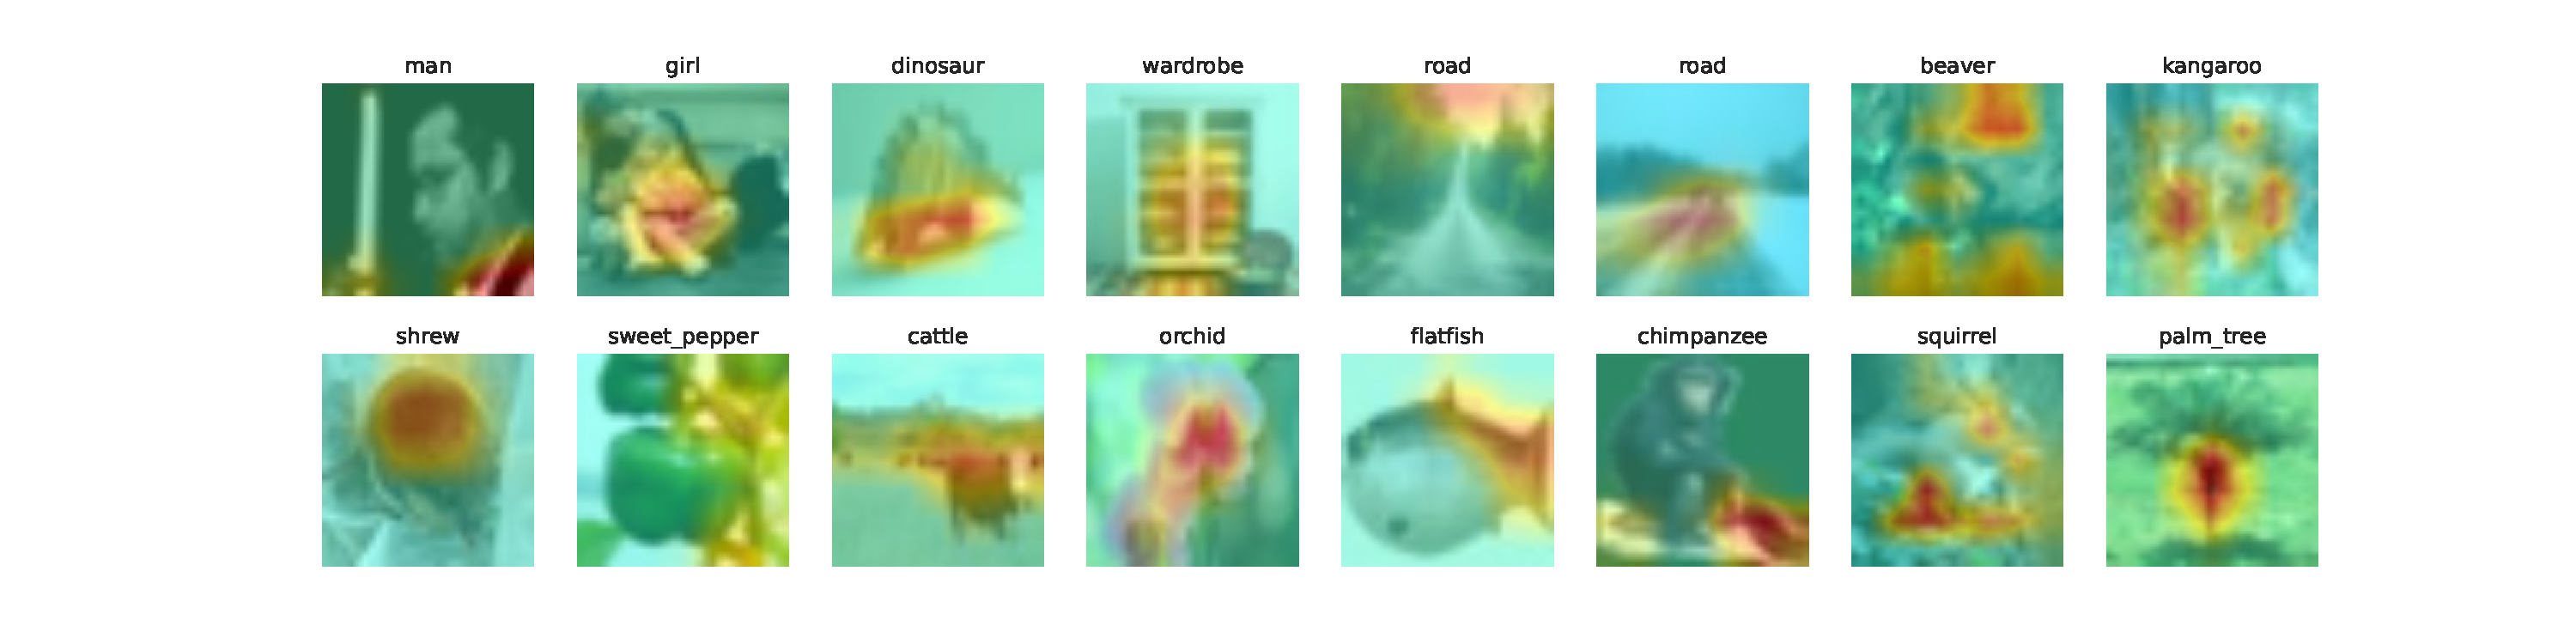
\includegraphics[width=\textwidth]{images/cifar100_efficientnet_b0_proxy_0.pdf}
            \caption{With Proxy Attention}
        \end{subfigure}
        \caption{Comparison of attention maps generated by efficientnet\_b0 trained with and without Proxy Attention on the cifar100 dataset}
    \end{figure}
    

    \begin{figure}[H]
        \centering
        \begin{subfigure}[b]{1\textwidth}
            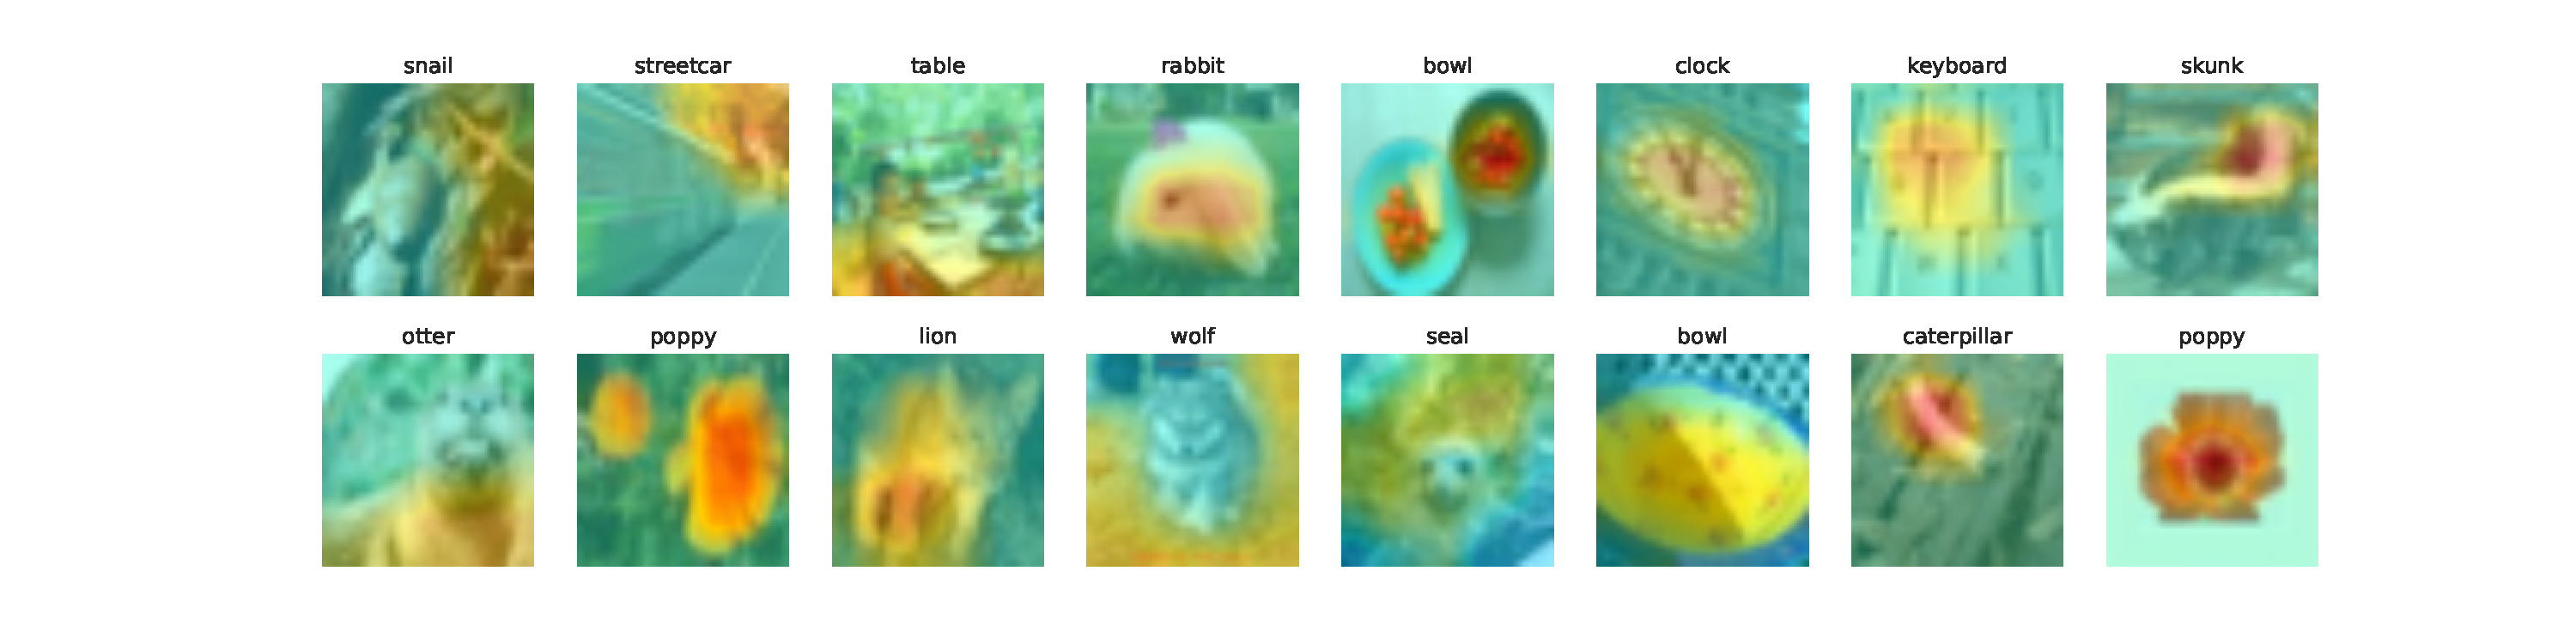
\includegraphics[width=\textwidth]{images/cifar100_efficientnet_b0_noproxy_0.pdf}
            \caption{Without Proxy Attention}
        \end{subfigure}
        \hfill
        \begin{subfigure}[b]{1\textwidth}
            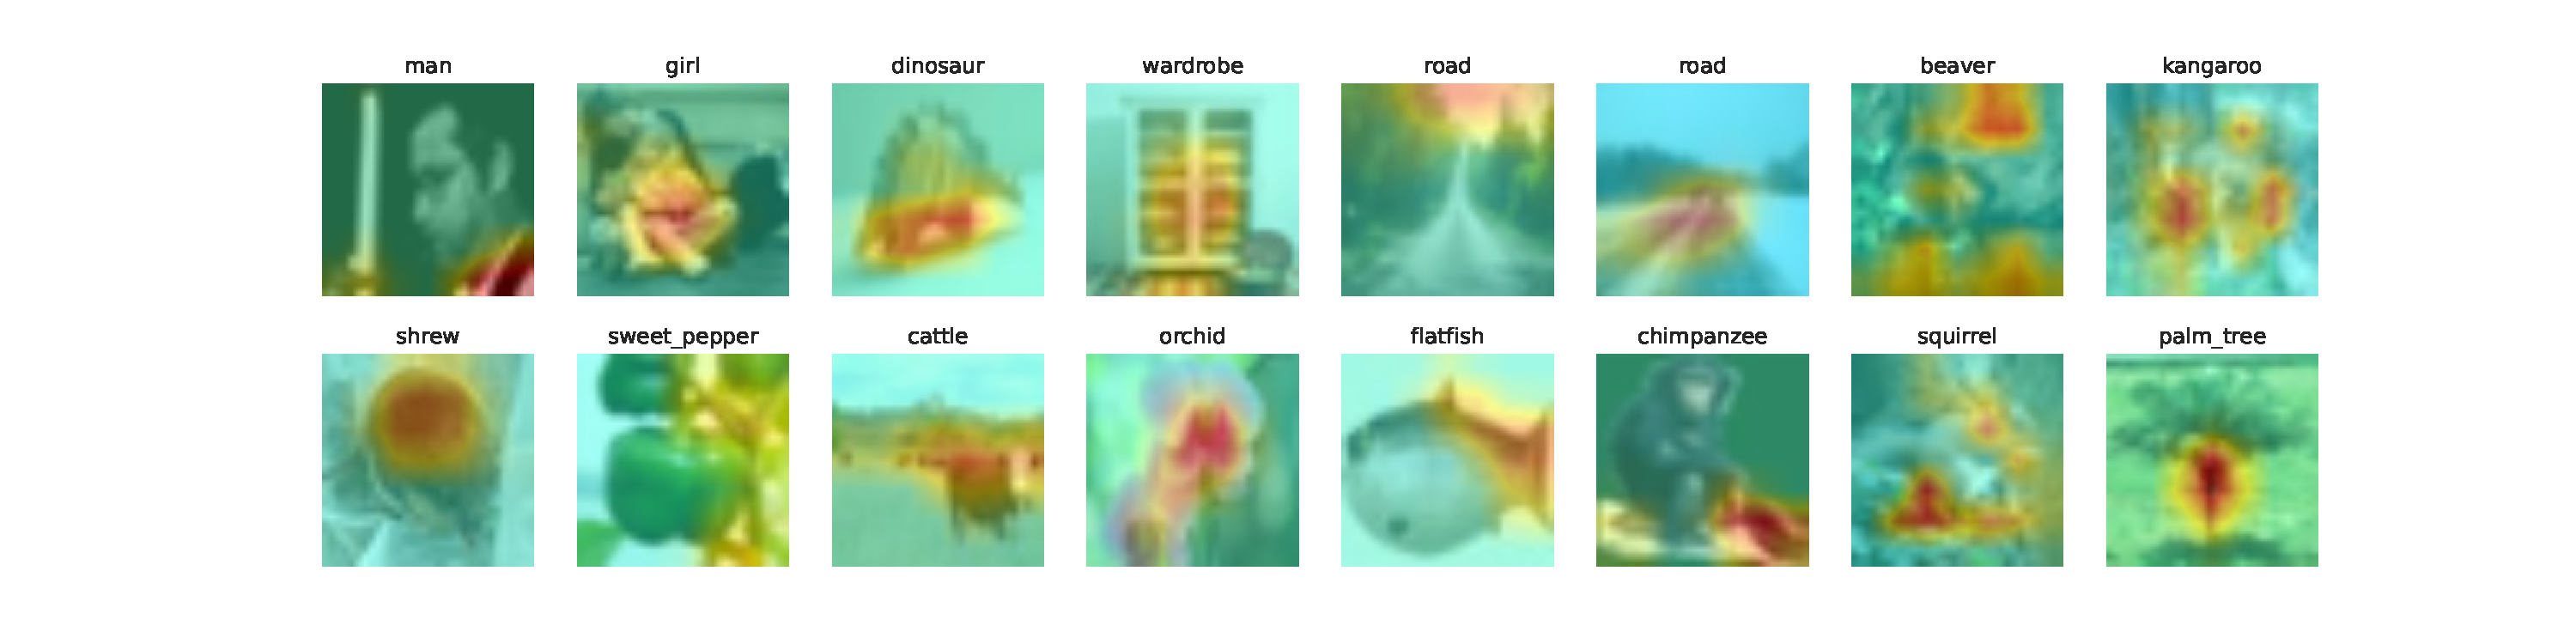
\includegraphics[width=\textwidth]{images/cifar100_efficientnet_b0_proxy_0.pdf}
            \caption{With Proxy Attention}
        \end{subfigure}
        \caption{Comparison of attention maps generated by efficientnet\_b0 trained with and without Proxy Attention on the cifar100 dataset}
    \end{figure}
    
